\documentclass[a4paper,12pt]{article}
\usepackage[utf8]{inputenc}
\usepackage{listings}
\usepackage{color}
\usepackage{url}
\usepackage{hyperref}
\definecolor{codegreen}{rgb}{0,0.6,0}
\definecolor{codegray}{rgb}{0.5,0.5,0.5}
\definecolor{codepurple}{rgb}{0.58,0,0.82}
\definecolor{backcolour}{rgb}{0.95,0.95,0.92}
\lstdefinestyle{Cstyle}{
	backgroundcolor=\color{backcolour},   
    commentstyle=\color{codegreen},
    keywordstyle=\color{magenta},
    numberstyle=\tiny\color{codegray},
    stringstyle=\color{codepurple},
    basicstyle=\footnotesize,
    breakatwhitespace=false,         
    breaklines=true,                 
    captionpos=b,                    
    keepspaces=true,                 
    numbers=left,                    
    numbersep=5pt,                  
    showspaces=false,                
    showstringspaces=false,
    showtabs=false,                  
    tabsize=2
}
\lstset{style=Cstyle}
\usepackage{tikz}
\usetikzlibrary{shapes.geometric, arrows}
\usepackage{xcolor}
\tikzstyle{startstop} = [rectangle, rounded corners, minimum width=3cm, minimum height=1cm,text centered, draw=black ]

\tikzstyle{io} = [trapezium, trapezium left angle=70, trapezium right angle=110, minimum width=3cm, minimum height=1cm, text centered, draw=black]

\tikzstyle{process} = [rectangle, minimum width=3cm, minimum height=1cm, text centered, draw=black ]

\tikzstyle{decision} = [diamond, minimum width=3cm, minimum height=5mm, text centered, draw=black]
\tikzstyle{arrow} = [thick,->,]
\usepackage{graphicx}
%\graphicspath{ {/home/shivamgupta/Pictures/} }
\usepackage{ragged2e}
\usepackage{geometry}
\renewcommand{\baselinestretch}{1.5}
\setlength{\parindent}{4em}
\usepackage{amssymb}
\begin{document}
\begin{center}
\textbf{Assignment-8 \\
\vspace{5mm}
ELP - 718 Telecom Software Laboratory \\
\vspace{2mm}
Shivam Gupta \\
2018JTM2774 \\
2018-2020} \\
\vspace{10mm}
A report presented for the assignment on \\
Python/Github \\
\vspace{30mm}

\includegraphics[scale=0.5]{iitlogo} \\
\vspace{10mm}
Bharti School Of \\
Telecommunication Technology and Management \\
IIT Delhi \\
India \\
September 27, 2018


\end{center}
\begin{flushleft}
\newpage
\tableofcontents

\section{\large{Problem Statement-1}} 
\subsection{Problem Statement}
IIT Delhi, has just got the strongest computer. The professors in charge wants to check the computational capacity of the computer. So, they decided to create the problem which is to be given as an assignment to students. Can you help the professor to check the computation capability of the computer?

A valid cross is defined here as the two regions (horizontal and vertical) of equal lengths crossing over each other. These lengths must be odd, and the middle cell of its horizontal region must cross the middle cell of its vertical region.
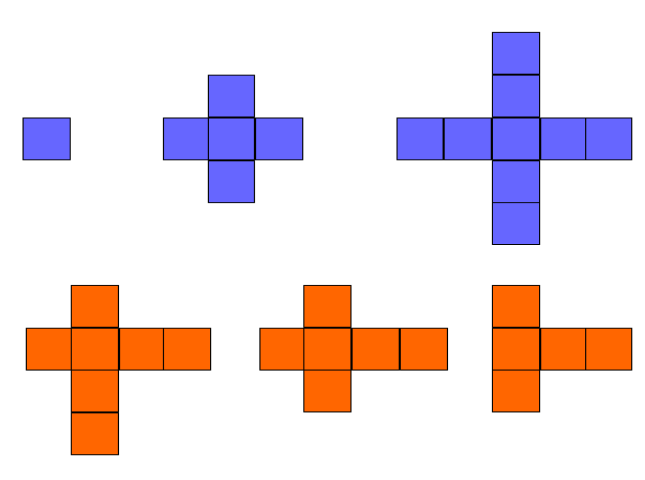
\includegraphics[scale=0.5]{ps1_1.png}\\
In the diagram above, the blue crosses are valid and the orange ones are not valid. 


Find the two largest valid crosses that can be drawn on smart cells in the grid, and return two integers denoting the dimension of the each of the two largest valid crosses. In the above diagrams, our largest crosses have dimension of 1,  5 and 9 respectively .\\

Note: The two crosses cannot overlap, and the dimensions of each of the valid crosses should be maximal.\\
Constraints\\
2 $<=$ n $<=$ 105\\
2 $<=$ m $<=$ 105\\



\subsection{Assumptions}
\begin{itemize}
\item we are using Python for implementing the code.
\item We are using Github to update file every hour.
\item Output is indicating by taking screenshots of the terminal.
\end{itemize}
\subsection{Program Structure}
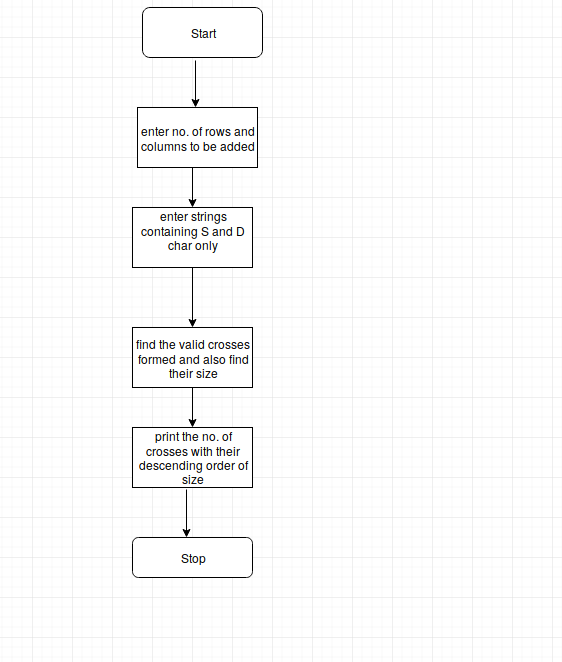
\includegraphics[scale=0.8]{flow1.png}
\subsection{Algorithm and Implementation}
\begin{itemize}
\item Create a ps1.py file through gedit editor and write a Python program on it to find the valid crosses.
\item After writing the program run it on terminal.
\item removing unnecessary errors during run time.
\item Take the screenshot of the final input. 
\end{itemize}
\subsection{Input and Output formats}
\textbf{Input Format} \\
The first line contains two space-separated integers,  n and m. 
Each of the next  lines n contains a string of  m characters where each character is either S (Smart) or D (Dull). These strings represent the rows of the grid. If the jth character in the ith  line is S, then  (i,j) is a  cell smart. Otherwise it's a  dull cell.\\

\textbf{Output Format} \\
Find two valid crosses that can be drawn on smart cell of the grid, and return the dimension of both the crosses in the reverse sorted order(i.e. First Dimension should be the larger one and other should be smaller one).\\
Sample Input 0\\
5 6\\
SSSSSS\\
SDDDSD\\
SSSSSS\\
SSDDSD\\
SSSSSS\\

Sample Output 0\\
5 1\\

Sample Output 1\\
6 6\\
DSDDSD\\
SSSSSS\\
DSDDSD\\
SSSSSS\\
DSDDSD\\
DSDDSD\\

Sample Output 1\\
5 5 (their can be more than one valid crosses of the same dimension, you can consider any.)\\
Sample Input 2\\
5 9\\
SSSSDSDDD\\ 
DDSDDDDDD\\
SSSSSDDDD\\
DDSDDSDDD\\
DSSSDDDDD\\

Sample Output 2\\
9 1\\





\subsection{Difficulties}
Error during compilation.
\subsection{Screenshots}
\begin{figure}
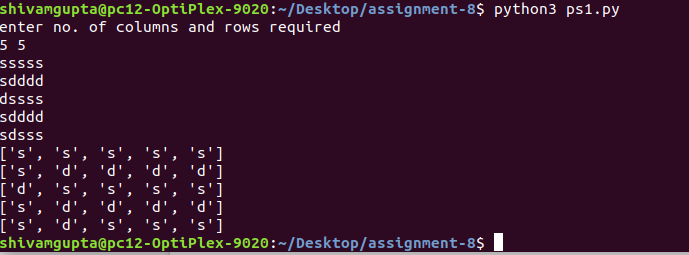
\includegraphics[scale=1]{ps1.png}
\caption{ps1}
\end{figure}
\newpage
\section{\large{Problem Statement-2}} 
\subsection{Problem Statement}
\begin{flushleft}
After, getting mix results of valid crosses, professors decided to test the computation abilities on one more problem. This time professors wanted to test the decryption capabilities of the computer.
Encryption of  a message requires three keys, k1, k2, and k3. The 26 letters of English and underscore are divided in three groups,  [a-i] form one group, [j-r] a second group, and everything else ([s-z] and underscore) the third group. Within each group the letters are rotated left by ki positions in the message. Each group is rotated independently of the other two. Decrypting the message means doing a right rotation by ki positions within each group.\\
Constraints\\
1 $<=$ Length of the string $<=$150\\
1$<=$ ki $<=$150 (i$=$1,2,3)\\


Explanation\\

Looking at the encrypted message, we see,
{d,i,h,e,e,c,c,e,h,a} appears at positions {1,2,4,10,14,15,18,26,27,28}, which after right rotation of given,\\
K1 = 2, these positions will contain the letters {h,a,d,i,h,e,e,c,c,e}.\\

Similarly, we can rotate other group letters by rotating right by the amount ki to get the decrypted message.\\



\end{flushleft} 
\subsection{Assumptions}
\begin{itemize}
\item we are using Python programming for implementing the code.
\item We are using Github to update file every hour.
\item Output is indicating by taking screenshots of the terminal.
\item Rotating letters in one group will not change any letters in any of the other groups.
\end{itemize}
\subsection{Program Structure}
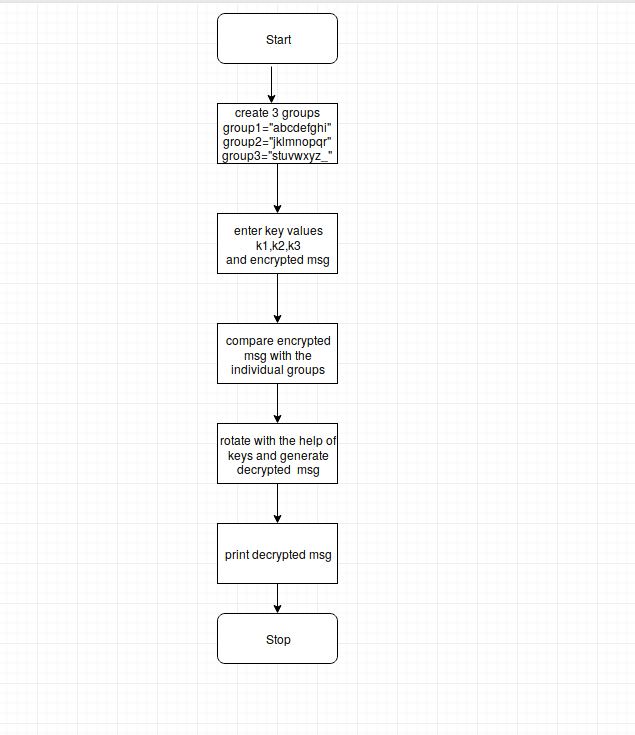
\includegraphics[scale=0.6]{flow2.png}
\subsection{Algorithm and Implementation}
\begin{itemize}
\item Create a ps2.py file through gedit editor and write a Python program on it.
\item After writing the program for decrypting the message run it on terminal.
\item Removing unnecessary errors during run time.
\item Now take screenshot of the final input.
\end{itemize}
\subsection{Input and Output formats}
\textbf{Input Format} \\
All input strings comprises of only lowercase English alphabets and underscores (-).\\
\textbf{Output Format} \\
For each encrypted message, the output is a single line containing the decrypted string\\
Sample Input 1\\
2 3 4\\
dikhtkor-ey-tec-ocsusrsw-ehas-\\

Sample Output 1\\
hardwork-is-thekey-to-success\\
Sample Input 2\\
1 1 1\\
bktcluajs\\

Sample Output 2\\
ajsbktclu\\




\subsection{Difficulties}
Run time errors.
\subsection{Screenshots}
\begin{figure}
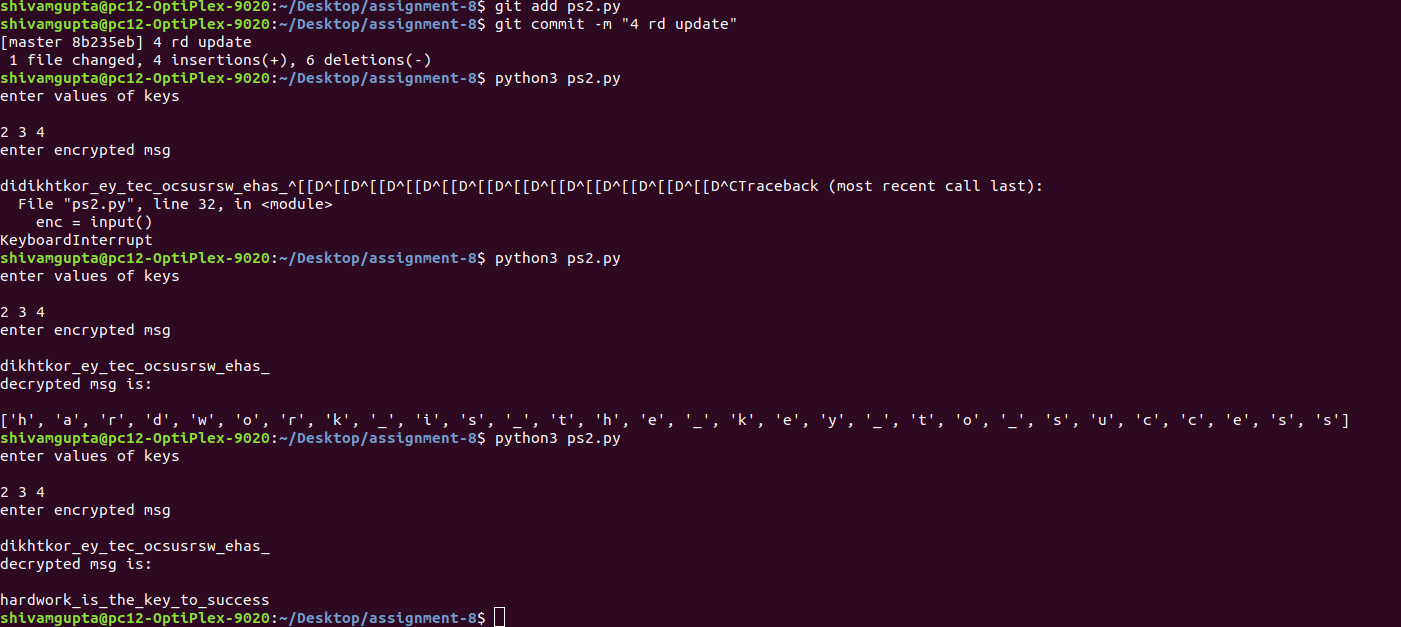
\includegraphics[scale=0.5]{ps2.png}
\caption{ps2}
\end{figure}
\newpage
\nocite{*}

\section{\large{Appendix}} 
\subsection{Source code for ps1}
\lstinputlisting[language=Python]{ps1.py}]
\subsection{Source code for ps2}
\lstinputlisting[language=Python]{ps2.py}]



\newpage
\bibliographystyle{plain}
\bibliography{report8.bib}
\end{flushleft}
\end{document}